\section{Evolutionary Analysis}

We performed two evolutionary experiments to characterize our five tag-matching metrics.
The first, in which we evolved sets of tags to form connectivity patterns matching a target graph, allowed us to isolate how tag-matching constraints (how many tag-matching criteria that must be simultaneously fulfilled) affected the rate of adpative evolution and the solution quality of evolved solutions.
The second, in which we evolved full-fledged SignalGP programs that used tag matching to control module activation, allowed us to investigate if tag-matching metrics exhibited different performance characteristics in a more generalized, complex domain.

\subsection{Matching a Target Graph}

In this evolutionary experiment, we evolved genomes consisting of 32 bitstring tags to establish a pattern of connectivity mirroring that of a randomly-generated target bipartite graph.
Each bitstring tag in a genome corresponded to a node in the target graph.
Half of the graph nodes, comprising one partition of the graph, were designated as queries.
The other half of the graph nodes, comprising the other partition of the graph, were designated as operands.
To evalute the fintess of a genome, we harvested the tags corresonding to the operand nodes of the graph and placed them into a tag-matching data structure.
This data structure allowed us to calculate the best matches among the set of operand tags for each query tag (the operand tags with minimal match distance to that query).
For each query tag, we recorded as many match results as outgoing connections from the corresponding node in the target graph.
Fitness was calculated as the fraction of operand tag results that corresponded to nodes in the target graph that queries connected to.

We controlled the amount of tag-matching constraint imposed by the target graph by manipulating:
\begin{enumerate}
  \item the mean number of edges per node (graph degree), and
  \item whether edges were assigned evenly such that all nodes had identical degree (regular structure) or were assigned at random, likely causing some nodes to have high degree (irregular structure).
\end{itemize}
We tested target graphs mean degree 1 and 2 and both regular and irregular construction.
Regular, degree 1 graphs imposed the least tag-matching constraint.
Degree 2 graphs imposed the most tag-matching constraint.
Supplementary Figure \ref{fig:graph_layouts} provides a visual depiction of these graph layouts.

For each target graph configuration, we surveyed each metric's performance over ten per-bit mutation rates ranging from 0.75 expected mutations per genome to 16.0 expected mutation rates per genome.
For each metric and target graph configuration combination, we chose the most favorable mutation rate defined by sum population-maximum fitness across updates.\footnote{
Supplementary Figure \ref{fig:evolve_mutsweep} summarizes evolutionary performance of metrics across mutation rate/target graph configurations.
All metrics show evidence of a performance maxima within the range of mutation rates surveyed, except for the hash metric on the regular target graph of degree 1 where peak performance was observed on the lowest sampled mutation rate.
}
We ran 100 replicate 512-generation evolutionary runs for each mutation rate/target graph/metric combination.
We used a well-mixed population of size 500 and tournament size 7.

\begin{minipage}{\linewidth}
\begin{center}

\begin{minipage}{\linewidth}
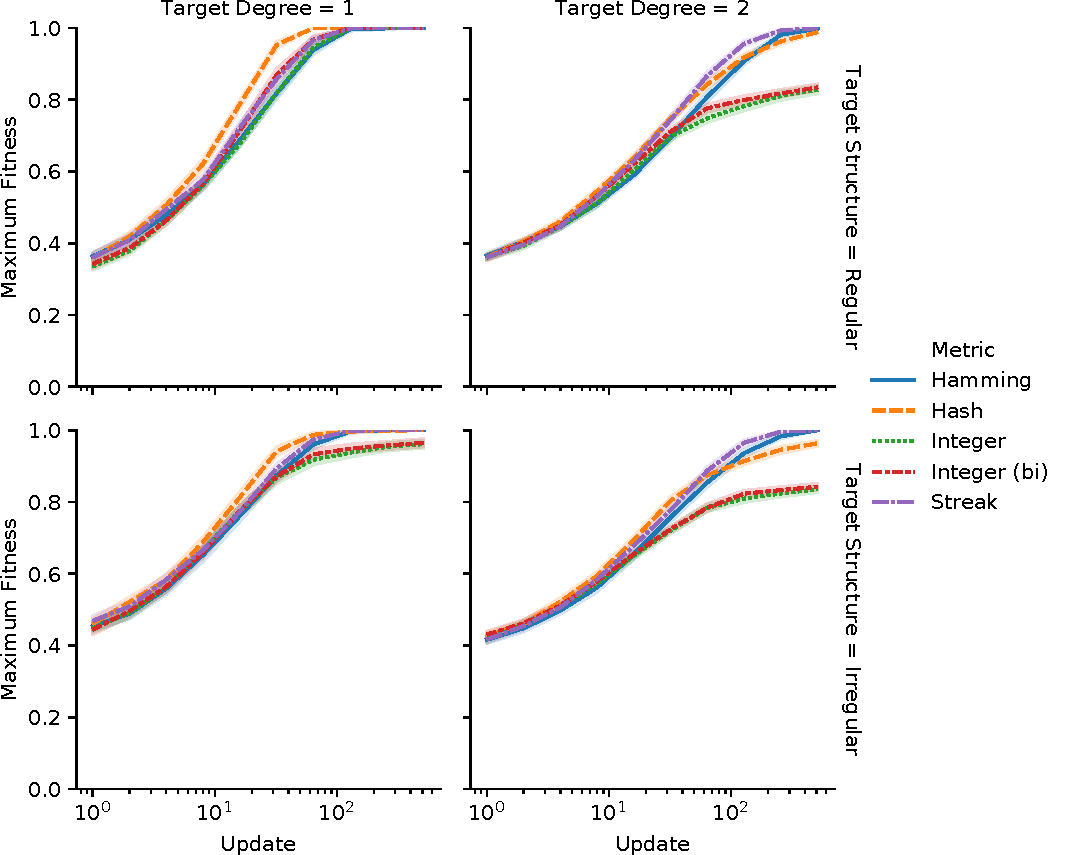
\includegraphics[width=\linewidth]{target_evolve/viz=max-fitness-line+_data_hathash_hash=673d309ab90e91d1+_script_fullcat_hash=fe3ddc711c5abfad+ext=}
\end{minipage}
\begin{minipage}{\linewidth}
\caption{
Maximum fitness by update over replicate runs for each metric's best-performing mutation rate.
Note log-scale x-axes.
Shaded area represents 95\% confidence intervals.
}
\label{fig:evolve_bests}
\end{minipage}
\end{center}
\end{minipage}


Figure \ref{fig:evolve_bests} plots population-maximum fitness across evolutionary runs.
The fitness trajectory of each metric under its best-performing mutation rate is shown.

Suprisingly, the hash metric enables faster adaptive evolution than all other metrics toward matching the least-constrained target graph, regular structure with mean degree 1 (non-overlapping 95\% CI).
On more-constrained target graphs with mean degree 2, the hash metric's advantage in rapid adaptive evolution dissappears.
In fact, on the most-constrained target graph (irregular structure with mean degree 2) the hash metric yields significantly lower-quality solutions at the end of evolutionary runs than the streak and hamming metrics.

The integer and bidirectional integer metrics successfully evolve connectivity patterns matching the unconstrained target graph (regular structure with mean degree 1) but yield lower-quality solutions than other metrics on constrained target graphs (non-overlapping 95\% CI).

The streak metric facilitates slightly faster adaptive evolution than the hamming metric, especially on mean degree 2 target graphs (non-overlapping 95\% CI).

We performed the same evolutionary experiment with 64-node target graphs and observed qualatively similar results (Supplementary Figure \ref{fig:evolve_bests64}).

\subsection{Evolving a Genetic Program}

% @AML: Once flow of paper, overall message, etc is decided, we'll most likely want to change this sub-heading
% @AML: Todo - update metric names to be consistent with rest of the paper.

\begin{figure*}
  \begin{center}

  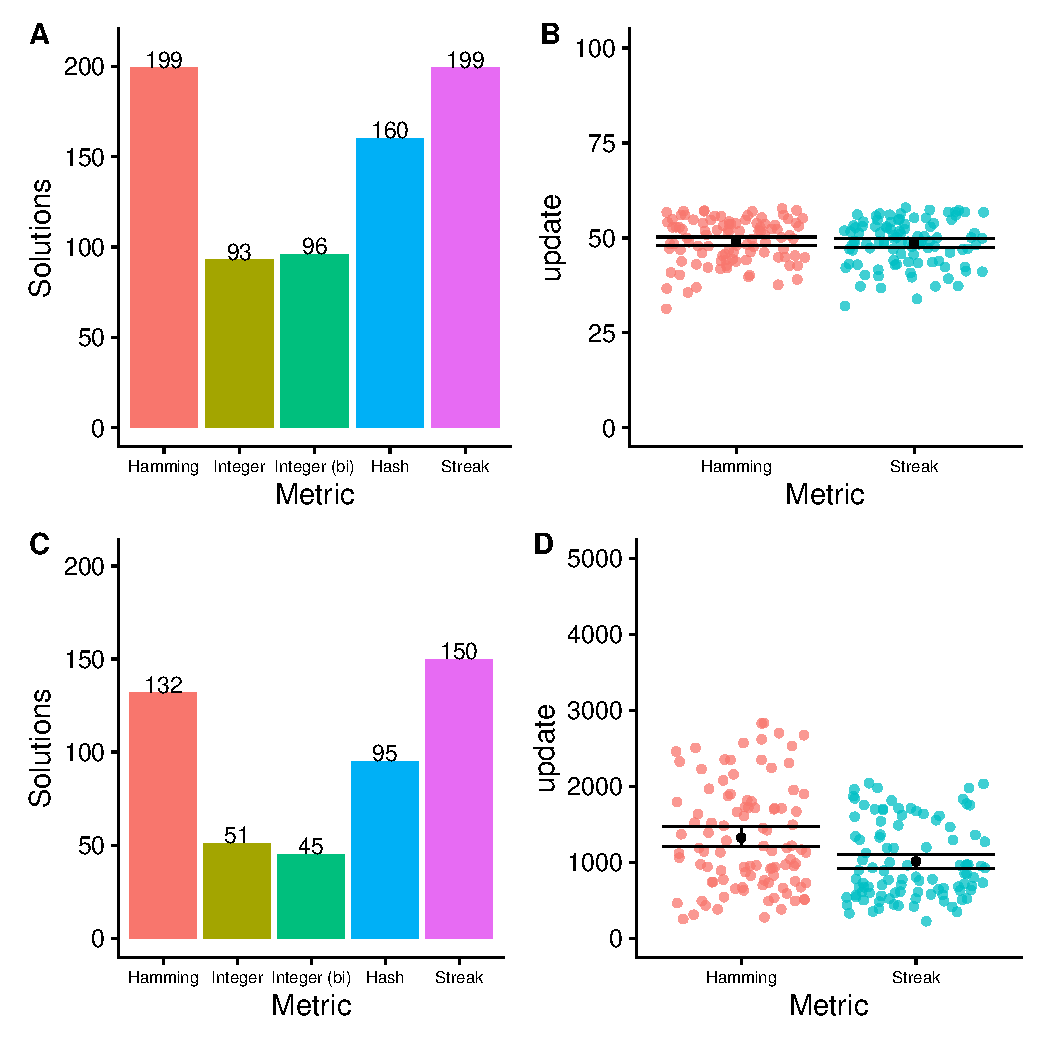
\includegraphics[width=\columnwidth]{img/gp_results/gp_results_panel}
  \caption{
  Todo - caption. A, B are changing-signal task; C, D are directional signal task.
  }
  \label{fig:gp_results}

  \end{center}
  \end{figure*}

Figure [X] gives the number of replicates that produced a successful SignalGP program (i.e., capable of achieving maximum fitness) for each tag-matching metric on both the changing- and directional-signal tasks.
For each task, we used a pairwise Fisher's exact test (with a Holm correction for multiple comparisons) to compare the number of successful replicates of each metric.
Our data and fully detailed statistical results are given in our supplemental material [cite - SGP supplement].

We observed no difference in success between the integer and integer-symmetric metrics on both the changing- and directional-signal tasks.
[Statement about consistency with expectations based on previous tag-matching experiments].
% - Appears to be consistent with results from graph matching evolution experiment. Needs confirmation, though.
% - Interesting that these two metrics seem to have fairly different geometric properties (because wrap-around vs no wrap-around), but have fairly similar variational properties.
% - For GP problems here, wrap-around vs no wrap around seems to not make a difference.

Across both tasks, the streak and hamming metrics performed significantly better than all other metrics ([STATS]).
On the changing-signal task, the hamming and streak metrics performed identically.
However, on the directional-signal task, the streak metric performed significantly better than the hamming metric ([STATS]).
To assess whether the streak metric produced solutions in fewer generations than the hamming metric, we re-ran 200 replicates of each condition (with new random number seeds) until a solution evolved in each of 50\% of the replicates (Figure [X]).
We found no difference between the hamming and streak metrics in the number generations elapsed before a solution to the changing-signal task evolves.
On the directional-signal task, however, we found that streak metric generally resulted required fewer generations for a solution to evolve than the hamming metric (Wilcoxon rank-sum test, $p < 0.0016$)
% TODO - double check that result in analyses
[Statement about consistency with expectations based on previous tag-matching experiments].
% Seems largely consistent with mean-degree-2 results (for later updates) in graph matching evolution experiment.
% More work to be done, but these data indicate that streak metric can be used for best/consistent performance in GP.

Surprisingly, the Hash metric performed well on both diagnostic tasks, outperforming both the integer and integer-symmetric metrics ([STATS?]).
The hash metric roughly maximizes the amount of phenotypic variation (i.e., signal-function relationships) that can be generated by mutating a single genotype --- a single bit flip in a tag is likely to completely re-order which other tags it best matches with.
The capacity to quickly generate large amounts of phenotypic variation allows evolution to explore a large swaths of the fitness landscape from generation to generation.
However, this capacity to generate phenotypic variation trades off with tag-matching robustness --- a single mutation to a tag is likely to destroy any established relationships with other tags.
Of each of the metrics we explored, the hash metric is the most susceptible to mutational meltdowns at high mutation rates.

% [Statement about consistency with expectations based on previous tag-matching experiments].
% [Statement about how Hash metric is good at exploring lots of combinations very quickly, with a low enough mutation rate].


% [Statement about these results overall in context of other results?].
% More work to be done, but these data indicate that streak metric can be used for best/consistent performance in GP.


